Hai thanh thẳng đồng chất, làm từ cùng vật liệu nở ra vì nhiệt, được nối đầu tại khớp quay A và C cố định trên tường thẳng đứng, và được nối với nhau tại khớp quay B cố định trên đầu và thân các thanh (xem hình vẽ đính kèm). Nhiệt độ của hệ đang tăng lên đều. Tại thời điểm được xét, khoảng cách $\overline{\text{AB}}=s_1$, $\overline{\text{CB}}=s_2$, $\overline{\text{AC}}=s_3$, $\overline{\text{BT}}=s_4$, và thành phần vận tốc của khớp B theo phương thẳng đứng là $v_{\parallel}$. Cho biết $s_1<s_2$, tường làm từ vật liệu không thay đổi kích thước vì nhiệt, hãy xác định vector vận tốc (phương chiều và độ lớn) của đầu thanh T khi ấy (theo $s_1$, $s_2$, $s_3$, $s_4$, và $v_\parallel$).

\begin{figure}[ht]
\centering
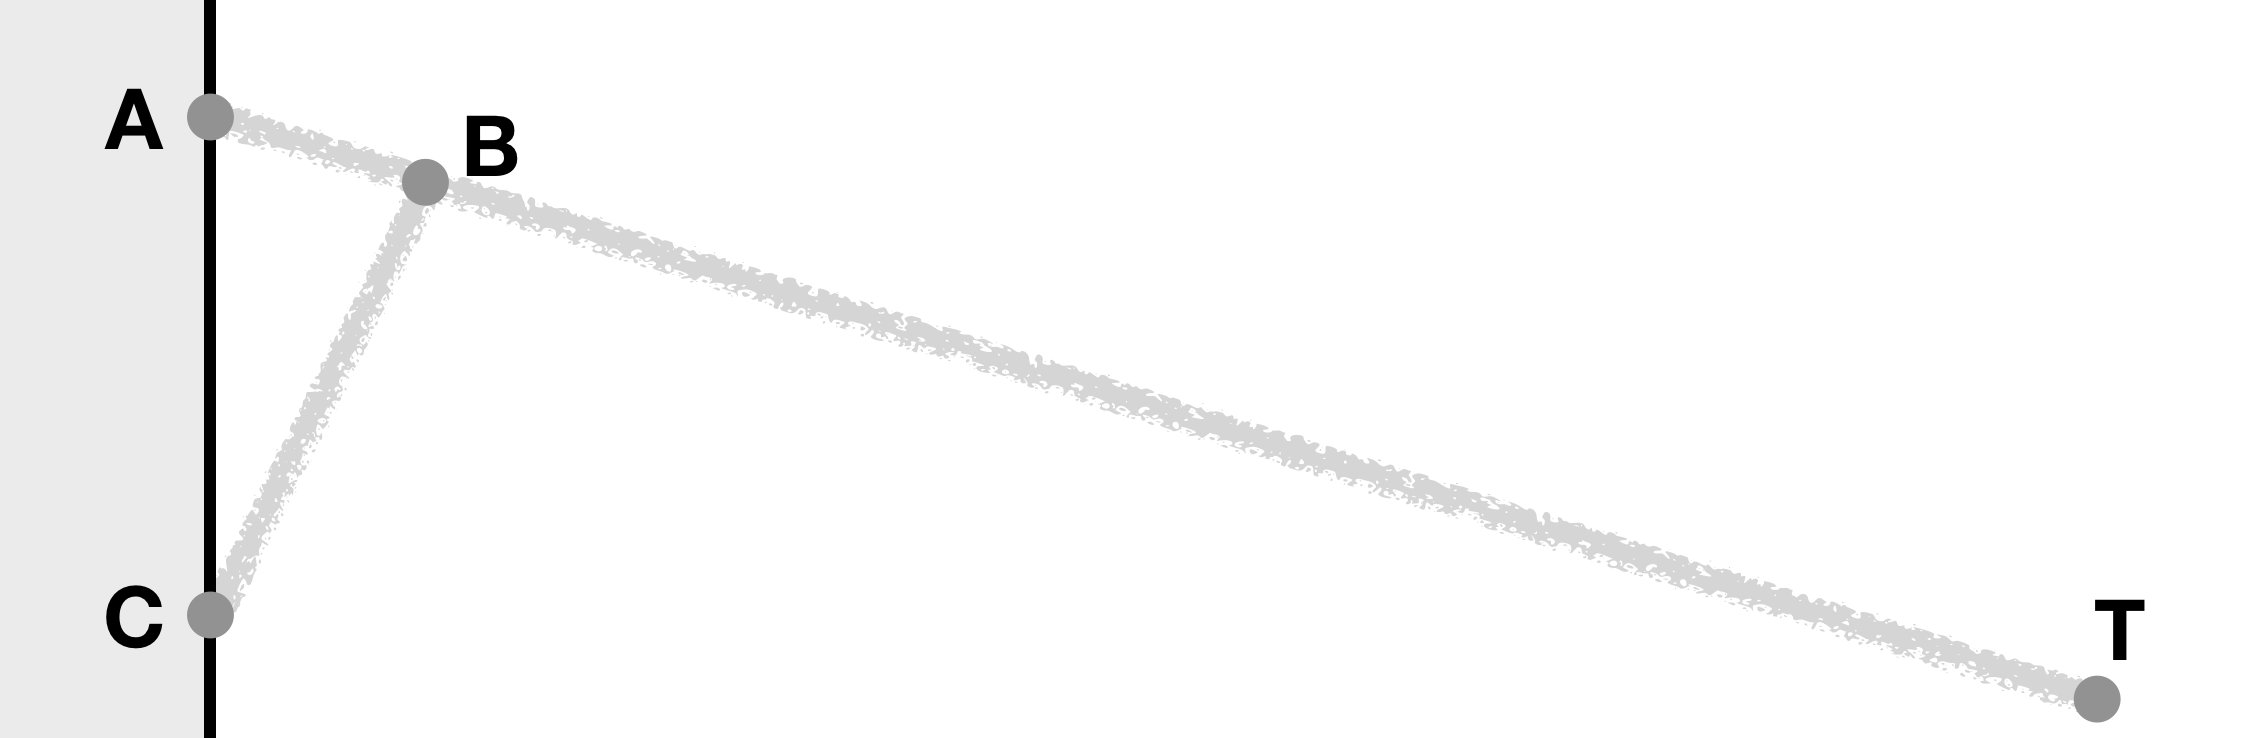
\includegraphics[width=0.7\textwidth,keepaspectratio]{Problem_3/Figs/P3.png}
\end{figure}